\documentclass[a4paper, 12pt]{article}
\usepackage[T1]{fontenc}
\usepackage[utf8]{inputenc}
\usepackage[english]{babel}
\usepackage{graphicx}
\usepackage[style=ieee, backend=biber]{biblatex}
%\usepackage[hidelinks]{hyperref}
\usepackage{hyperref}
\addbibresource{bib.bib}
\usepackage{setspace}
\usepackage{amsfonts}
\usepackage[nottoc,numbib]{tocbibind}
\usepackage{amsmath}
\numberwithin{equation}{section}

\onehalfspacing

\begin{document}

\title{Flatland Challenge}
\author{G. Berselli, R. De Matteo, M. M. L. Pulici}
\date{July 19, 2021}
\maketitle
\begin{center}
	\fbox{
\includegraphics[width=\textwidth]{Images/Flatland_Logo.jpg}}
\end{center}


\clearpage

\tableofcontents

\clearpage


\section{Introduction}

\subsection{Flatland Challenge}

The aim of the challenge \cite{flatland}, is to achieve efficient management of railway traffic. In particular, this problem is tackled in a simple grid world environment, in order to simulate and experiment different scenarios.

In more detail, the goal consists in making a number of trains arrive at their destinations minimizing the travel time. Even though for simple environments the train can follow explicit plans, as complexity increases the problem of mapping all possible states becomes intractable, for this reason a class of algorithms known as Reinforcement Learning (Section \ref{ch:reinforcement-learning}) can be exploited.

\begin{figure}[h]
	\centering
		\fbox{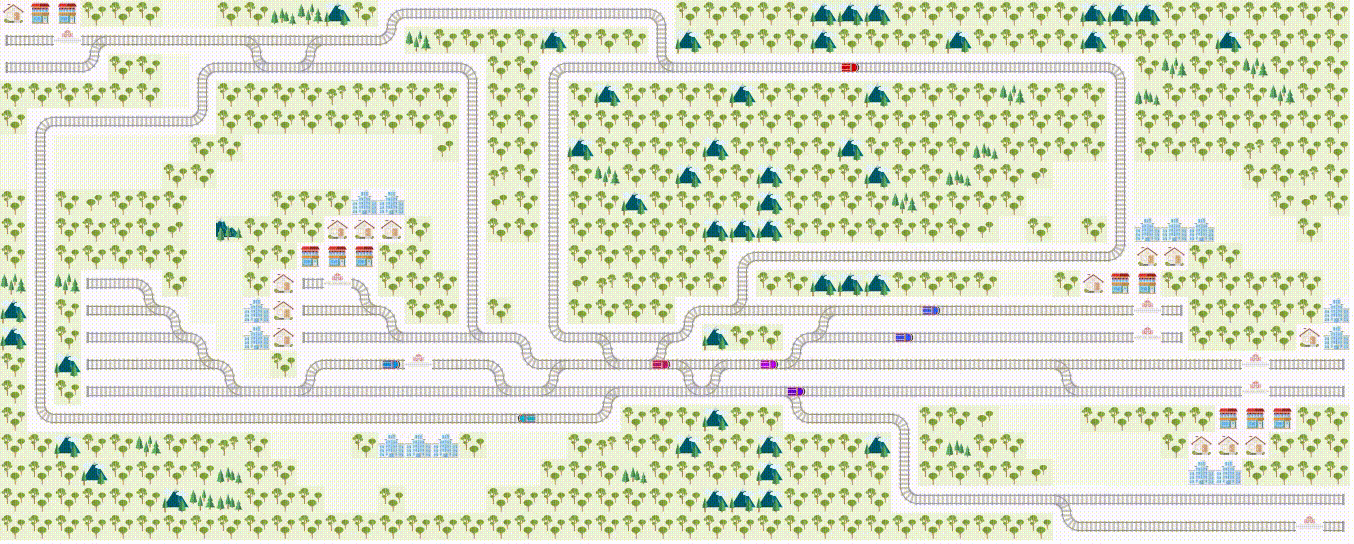
\includegraphics[width=\textwidth]{Images/Flatland_Example.png}}
		\caption{A possible Flatland instance.}
\end{figure}

\subsubsection{The environment}

The Flatland environment \cite{flatland-challenge} consists in a discrete time simulation, meaning that each action is performed with a constant time step. At each step, an agent for each simulated train chooses an action. An agent is defined as ``an entity that can move within the grid and must solve tasks'' \cite{flatland-challenge}. More precisely, each agent can choose between two actions: waiting or moving in a direction. Each agent has an individual starting position and its goal is to reach its target destination. Of course, two agents can not occupy the same cell at the same time.

Each cell in the Flatland grid can take the form of any of 8 tile types, as shown in Fig. \ref{fig:cell-types}. More configurations can be obtained by rotating and mirroring the 8 basic tiles.

\begin{figure}[h]
	\centering
		\fbox{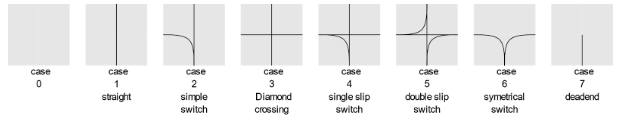
\includegraphics[width=\textwidth]{Images/cell-types.png}}
		\caption{The 8 cell types.}
	\label{fig:cell-types}
\end{figure}

When the tile is of the straight type, the agent can only choose to continue moving or to stop. In presence of a simple or a double switch, the train is forced to decide in which of the offered direction to move. When arriving at a dead end, an agent can only stop or go backward.


\subsection{Reinforcement Learning}\label{ch:reinforcement-learning}

The term Reinforcement Learning \cite{reinforcement-learning} refers to the class of agents which rely on feedbacks, or rewards, produced by the agents themselves when interacting with the environment. The way Reinforcement Learning works is to use observed rewards to learn the best possible policy for the given environment. In other words, the agent has no prior knowledge of the environment and must learn how to behave based only on posterior trial-and-error feedbacks.

There are three basic agent designs for Reinforcement Learning:
\begin{itemize}
	\item Utility-based agent, which learns a utility function on states and uses it to select actions;
	\item Q-learning, which learns an action-utility function giving the expected utility of an action given a state;
	\item Reflex agent, which learns a policy mapping directly from states to actions.
\end{itemize}

In addition to these designs, Reinforcement Learning can be either passive, meaning that the policy is fixed and the task is to learn the utilities of states, or active, referring to agents which must also learn how to act.

\subsubsection{Q-learning}

For the Flatland Challenge, Q-learning is used. This class of algorithms learns an action-utility representation instead of simply learning the utilities. The value of an action-state tuple is typically indicated as $Q\left(s,a\right)$. There is a direct correlation between Q-values and state utilities, as expressed by the following equation:
\begin{equation}
	U\left(s\right) = \max_a Q\left(s,a\right).
\end{equation}

The main difference between Q-functions and basic utility information si that no model of the form $P\left(s'|s,a\right)$ is needed, either for learning or for action selection. This characteristic makes Q-learning a model-free method.

At equilibrium, when the Q-values are correct, the following equation must hold:
\begin{equation}\label{eq:equilibrium}
	Q\left(s,a\right)=R\left(s\right)+\gamma\sum_{s'}P\left(s'|s,a\right)\max_{a'}Q\left(s',a'\right).
\end{equation}

The issue with this approach is that the model of state transitions $P\left(s'|s,a\right)$ needs to be learned as well. To solve this problem, the so-called temporal-difference approach can be used. It consists in updating the Q-value every time an action is executed, using the following equation:
\begin{equation}\label{eq:TD-Q-learning}
	Q\left(s,a\right) \leftarrow Q\left(s,a\right) + \alpha\left(R\left(s\right)+\gamma\max_{a'}Q\left(s',a'\right)-Q\left(s,a\right)\right).
\end{equation}

A close alternative to Q-learning can be found in the \textsc{Sarsa} (State-Action-Reward-State-Action) algorithm. The concept is very close to that of Q-learning, but Eq. \eqref{eq:TD-Q-learning} is replaced by:
\begin{equation}\label{eq:SARSA}
	Q\left(s,a\right) \leftarrow Q\left(s,a\right) + \alpha\left(R\left(s\right)+\gamma Q\left(s',a'\right)-Q\left(s,a\right)\right).
\end{equation}

The only difference between Eqs. \eqref{eq:TD-Q-learning} and \eqref{eq:SARSA} is that $\max_{a'}Q\left(s',a'\right)$ is simply replaced by $Q\left(s',a'\right)$. In other words, instead of the maximum of the possible Q-values from the state reached in the transition, the actual value of the state $s'$ reached after taking action $a'$ is used. The value update takes place once at the end of each $s$, $a$, $r$, $s'$, $a'$ cycle, as suggested by the name.

If the agent is a greedy one, always choosing the action with the best Q-value, there is no difference between the two algorithms. If, on the other hand, there is some exploration happening, there is a crucial difference: Q-learning is said to be an off-policy algorithm, because it does not care about the policy used; \textsc{Sarsa}, on the contrary, is considered on-policy. Even though Q-learning is more flexible, being able to learn well even with bad exploration policies, it is not as realistic, since it does not take into consideration possible external uncontrollable events.

\subsubsection{Multi-Agent Reinforcement Learning}

Multi-Agent Reinforcement Learning (\textsc{Marl}) \cite{multi-agent-rl} refers to a version of Reinforcement Learning where multiple agents interact in a common environment. There are three main broad categories which classify \textsc{Marl}:
\begin{itemize}
	\item Cooperative: when all agents have a common goal and work together;
	\item Competitive: when agents compete to accomplish a goal;
	\item Mixed: when agents are grouped in teams, with intra-group cooperation and inter-group competition.
\end{itemize}



\section{Implementation}


\subsection{Observation}

\subsubsection{Predictor}


\subsection{Deep Q-Network Agent}

Learning using Deep Q-Networks (DQN) \cite{improvements} is a relatively new paradigm, having been introduced in 2014. In general, the main feature of DQN algorithms is the exploitation of Deep Neural Networks to learn the Q-values of a problem. There are many versions of DQN algorithms, of which the most common are:
\begin{itemize}
	\item Fixed Q-targets;
	\item Double DQN;
	\item Dueling DQN.
\end{itemize}

\begin{figure}[h]
	\centering
		\fbox{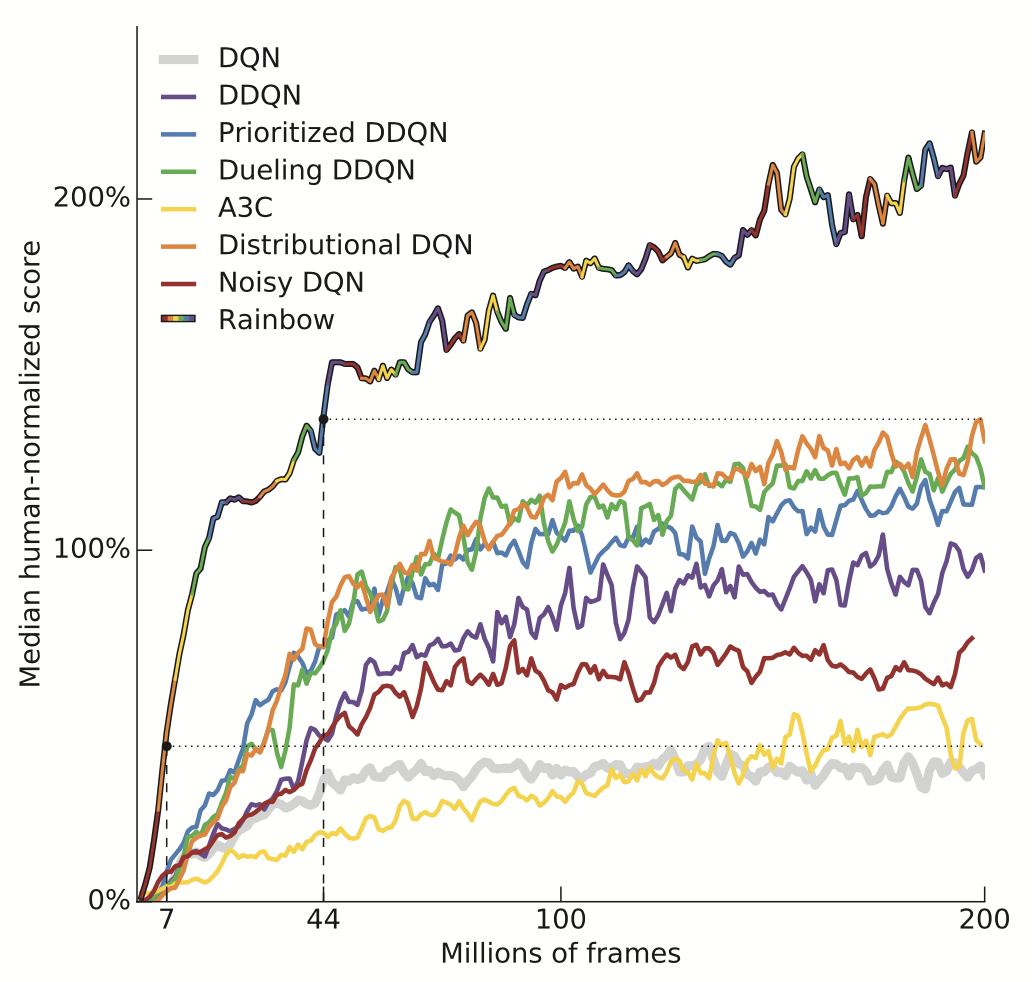
\includegraphics[width=\textwidth]{Images/rainbow.png}}
		\caption{Comparison of various DQN approaches, including the state-of-the-art Rainbow agent.}
	\label{fig:rainbow}
\end{figure}



\subsubsection{Fixed Q-targets}

When Eq. \eqref{eq:equilibrium} is used in a Neural Network, the same parameters are used for estimating both the target and the Q-value. This is an issue, since it means that there is a big correlation between the target and the changing parameters: at every step, both the Q-values and the target values shift, leading to big oscillations in training.

A possible solution is to use fixed Q-targets, meaning that a separate network is created with a fixed parameter for estimating the target. Every $\mathrm{T}$ steps, the parameters are copied from the DQN to update the target network. This way, learning becomes more stable because the target function stays fixed for some time.

\subsubsection{Double DQN}

An alternative to simple Fixed Q-targets is the so-called Double DQN. The aim of this approach is to tackle the problem of checking that the best action for the next state is the one with the highest Q-value. In general, the accuracy of Q-values depend on both the action chosen and what states have been explored. Therefore, at the beginning of the training there is no information about the best action to take: taking the maximum Q-value can lead to false positives. This natural tendency of DQN to given higher Q-values to suboptimal actions complicates learning.

The Double DQN approach tries to fix this problem by using two separate networks to decouple the action selection from the target Q-value generation. First, the DQN network is used to select the best action to take for the next state, then the target network calculates the target Q-value of the state-action combination. So, the Double DQN method reduces Q-value overestimation and makes training faster and stabler.

\subsubsection{Dueling DQN}

The third DQN version is based on decomposing the Q-value in two parts:
\begin{equation}
	Q\left(s,a\right)=V\left(s\right)+A\left(s,a\right)
\end{equation}
where $V\left(s\right)$ is the value of being in state $s$ and $A\left(s,a\right)$ is the advantage of taking action $a$ at state $s$. Dueling DQN focuses on separating the estimator of the two values, using one stream to estimate the state value $V\left(s\right)$ and another one to estimate the advantage of each action $A\left(s,a\right)$. Decoupling these two values becomes particularly useful for states where any action does not affect the environment in a relevant way.

\subsubsection{Further DQN approaches}

Of course, these three methods are not the only ones to deal with DQNs. A particularly exhaustive analysis of all the different improvements to the DQN algorithm is represented by the seminal work by Hessel et al. \cite{rainbow}: in the paper, different DQN approaches are compared, culminating in the creation of a state-of-the-art integrated ``Rainbow'' agent, exploiting all the advantages of the most successful approaches. These results are shown as a reference in Fig. \ref{fig:rainbow}.





\subsection{Proximal Policy Optimization}
Proximal Policy Optimization (PPO) \cite{ppo-algorithm}, \cite{understanding-ppo} is a technique designed to alternate between sampling data through interaction with the environment and optimizing an objective function using stochastic gradient ascent. The main feature of PPO is the use of the clipped surrogate objective:
\begin{equation}
	L^\mathrm{CLIP}\left(\theta\right)=\hat{\mathbb{E}}_t\left[\min\left(r_t\left(\theta\right)\hat{A}_t,\mathrm{clip}\left(r_t\left(\theta\right),1-\varepsilon,1+\varepsilon\right)\hat{A}_t\right)\right].
\end{equation}

Expectations are computed over a minimum of two terms: a normal objective and a clipped objective. Because of the $\min$ operator, the clipped objective behaves differently when the advantage estimate is positive or negative.

\begin{figure}[h]
	\centering
		\fbox{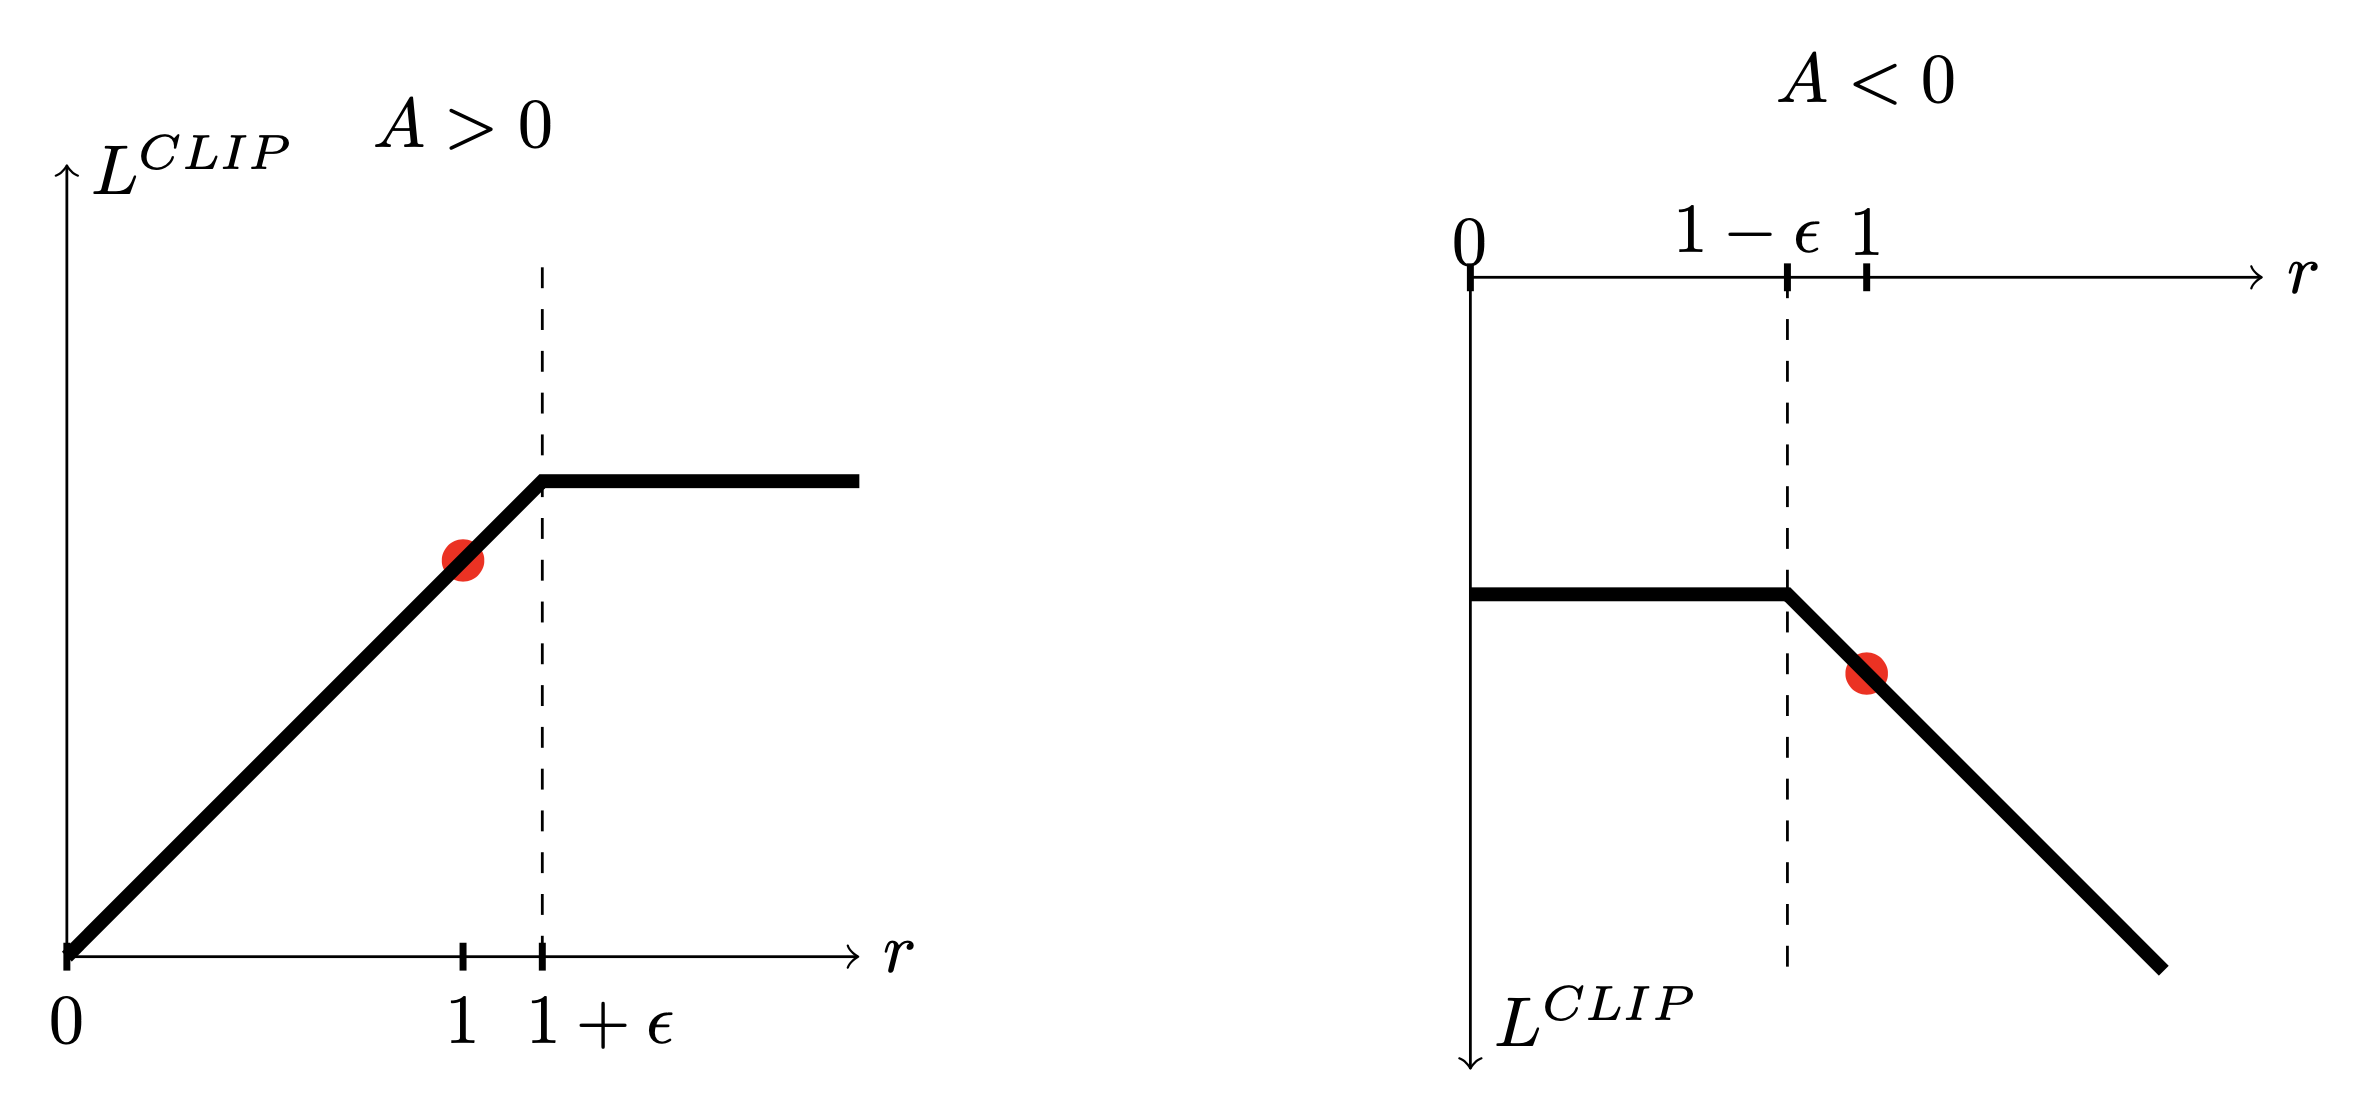
\includegraphics[width=\textwidth]{Images/clipped.png}}
		\caption{The $L^\mathrm{CLIP}$ function for positive advantages $A>0$ and negative advantages $A<0$. The red circles show the starting points for the optimization.}
	\label{fig:clipped}
\end{figure}

The effect of clipping is shown in Fig. \ref{fig:clipped}. On the left situation, when the selected action has a better-than-expected effect, the loss function flattens out when the action is much more likely under the current policy compared to the old one. This is done to prevent overdoing an action update by taking a step too far. The same happens to the graph on the right: the loss function flattens out when the action is much less likely under the current policy.




\subsection{Action Selectors}
In the learning process of a Reinforcement learning agent, exploration \cite{action-selectors} plays a crucial role: in order for an agent to properly learn from the interaction with the environment, it must be exposed to as many states as possible. Since an agent needs the right experiences to learn a good policy, but also needs a good policy to obtain the environment, a balance, known as exploration-exploitation tradeoff, needs to be reached. There are various action selection approaches which can be used by the agent, of which the main ones are:
\begin{itemize}
	\item Greedy Approach;
	\item Random Approach;
	\item $\varepsilon$-Greedy Approach;
	\item Boltzmann Approach;
	\item Noisy Approach.
\end{itemize}


\subsubsection{Greedy Approach}

The Greedy Approach is the most basic method of selecting an action. It consists in always opting for the action with the highest Q-value, regardless of the values of the other choices. This approach is illustrated in Fig. \ref{fig:greedy}.

\begin{figure}[h]
	\centering
		\fbox{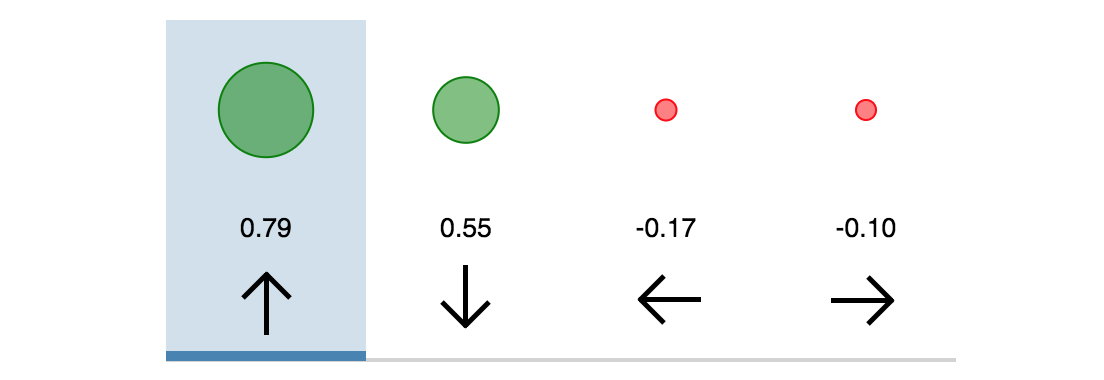
\includegraphics[width=\textwidth]{Images/greedy.png}}
		\caption{Action selection distribution for the Greedy Approach.}
	\label{fig:greedy}
\end{figure}

At first, this approach might appear good, as the agent always opts for the action it thinks to be the best. The main shortcoming of this method is that it almost always provides a suboptimal solution, since no alternate solutions are explored. In other words, in Greedy Approach, exploitation is favored enormously over exploration, which is almost absent. 


\subsubsection{Random Approach}

The Random Approach is the extreme opposite of the Greedy one: instead of always checking for the best Q-value, the agent does not look at Q-values at all, picking randomly among all the possible actions. This approach is illustrated in Fig. \ref{fig:random}.

\begin{figure}[h]
	\centering
		\fbox{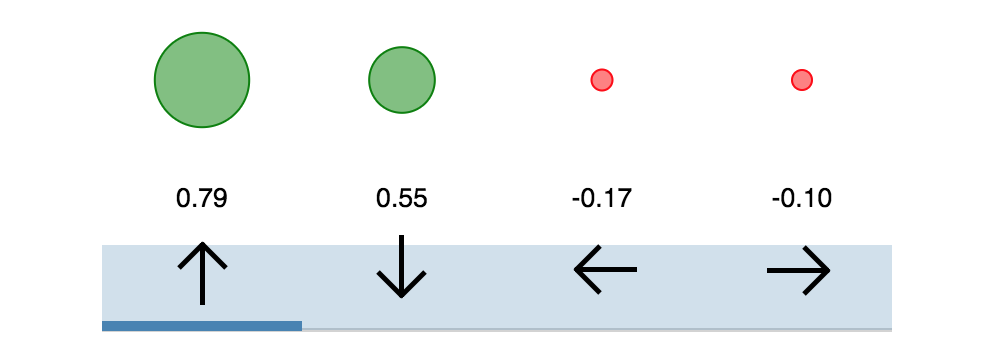
\includegraphics[width=\textwidth]{Images/random.png}}
		\caption{Action selection distribution for the Random Approach.}
	\label{fig:random}
\end{figure}

Despite providing a lot of exploration, this approach is obviously deficient in exploiting the knowledge already learned by the agent.


\subsubsection{$\varepsilon$-Greedy Approach}

The $\varepsilon$-Greedy Approach can be viewed as a combination of the Greedy and the Random ones. The way the agent acts in this case is by always opting for the optimal action, except occasionally it acts randomly. The choice between the two approaches is dictated by an adjustable parameter $\varepsilon$, which represents the probability to act randomly. This approach is illustrated in Fig. \ref{fig:epsilon}.

\begin{figure}[h]
	\centering
		\fbox{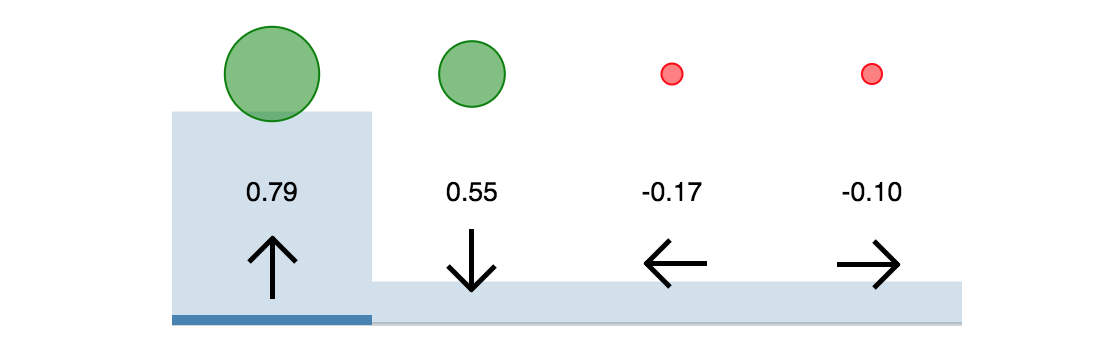
\includegraphics[width=\textwidth]{Images/epsilon.png}}
		\caption{Action selection distribution for the $\varepsilon$-Greedy Approach.}
	\label{fig:epsilon}
\end{figure}

This approach encountered a huge success due to its combination of simplicity and power: even though it is only a mixture of two very mediocre methods, the performance improvement is remarkable. To further enhance the agent's learning ability, the value of $\varepsilon$ is often adjusted during training: in the beginning it starts as a big value, in order to provide maximum exploration, and it is slowly annealed as the agent obtains more information about the environment. The only shortcoming of the $\varepsilon$-Greedy Approach is that it only takes into account whether an action is the most rewarding or not, making it not optimal.


\subsubsection{Boltzmann Approach}

The Boltzmann Approach takes the exploration-exploitation balance of $\varepsilon$-Greedy even further: instead of always taking the optimal action or acting randomly, it chooses among the various actions using individual Q-values to weigh probabilities. This approach is illustrated in Fig. \ref{fig:boltzmann}.


\begin{figure}[h]
	\centering
		\fbox{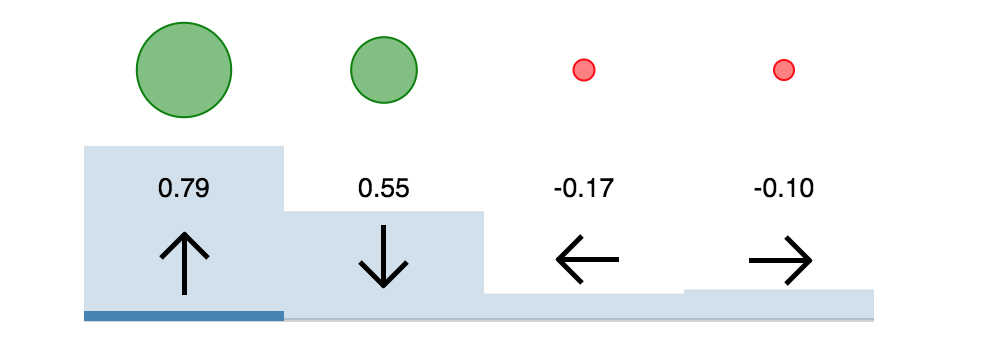
\includegraphics[width=\textwidth]{Images/boltzmann.png}}
		\caption{Action selection distribution for the Boltzmann Approach.}
	\label{fig:boltzmann}
\end{figure}

Compared to $\varepsilon$-Greedy, the Boltzmann Approach also takes into consideration the information about the values of actions other than the optimal: this way, actions which are potentially promising are given a higher priority over clearly inferior choices.

An interesting feature of the Boltzmann Approach is the use of an additional temperature parameter $\tau$, which is annealed over time in a fashion similar to the way $\varepsilon$ is treated. The $\tau$ parameter controls the probability distribution of the actions using the thermodynamics Boltzmann equation, which gives the name to the approach:
\begin{equation}\label{eq:boltzmann}
	P\left(a\right) = \frac{\mathrm{e}^\frac{Q\left(a\right)}{\tau}}{\sum_{i=1}^n \mathrm{e}^\frac{Q\left(a_i\right)}{\tau}},
\end{equation}
where $P\left(a\right)$ is the probability of choosing action $a$, and $a_i$ are all the possible action choices.

The main problem of this approach is that it builds on the assumption that the probability distribution outlined in Eq. \eqref{eq:boltzmann} provides a measure of the agent's confidence in action $a$, while in reality what the agent is estimating is a measure of how optimal the agent thinks the action is, not how certain it is about that optimality.



\subsubsection{Noisy Approach}

The Noisy Approach \cite{deep-reinforcement} is somewhat different from all the others: instead of acting on the probability of the agent choices, it adds some noise to the output of the Neural Network itself. In general, the weights $W_i$ are what the neural network needs to learn. Using the Noisy Approach, each weight can be expressed by the formula:
\begin{equation}
	W_i = \mu+\sigma\cdot\varepsilon
\end{equation}
where $\mu$ is a variable with random initialization, $\sigma$ is a variable with constant initialization, and $\varepsilon$ is the noise with a random value between $0$ and $1$.


\subsection{Experience Replay}

\subsubsection{Prioritized Experience Replay}
Prioritized Experience Replay \cite{prioritized-experience-replay} is a type of experience replay which consists in giving priority to transitions with high expected learning progress, measured by their temporal-difference error. This approach leads to two issues: firstly, the prioritization can produce a loss of diversity; secondly, it can introduce some bias.

The diversity loss problem can be solved by employing stochastic prioritization, a sampling method which interpolates between pure greedy prioritization and uniform random sampling: on the one hand, it ensures a monotonic sampling probability in a transition's priority; on the other hand, even the lower-priority transitions are guaranteed a non-zero probability. Practically, the probability of sampling a transition $i$ is given by:
\begin{equation}
	P\left(i\right)=\frac{p_i^\alpha}{\sum_kp_k^\alpha},
\end{equation}
where $p_i$ is the priority of transition $i$ and $a$ is the amount of prioritization which is used.

The introduction of a bias can be corrected by using importance-sampling weight, given by:
\begin{equation}
	w_i=\left(\frac{1}{N}\cdot\frac{1}{P\left(i\right)}\right)^\beta,
\end{equation}
which fully compensates for the non uniform probabilities if $\beta=1$. For stability reasons, weights are normalized by $\frac{1}{\max_iw_i}$, si that they only scale the update downwards.



\section{Results}

Experiment tracking was performed using the Weights and Biases tool \cite{wandb}.


\section{Conclusion}




















\clearpage
\printbibliography[heading=bibintoc]

\end{document}